
%%% Local Variables: 
%%% mode: latex
%%% TeX-master: t
%%% End: 


\title{Tipos Genéricos}

\frame{\maketitle}

\begin{frame}[fragile]{Antes dos genéricos}
  \begin{itemize}
  \item Todas as classes herdam por padrão os atributos e métodos da
    classe {\tt \alert{Object}};
  \item Uso da classe {\tt \alert{Object}} para lidar com a manipulação de
    tipos de objetos não conhecidos em tempo de compilação.
  \end{itemize}

\end{frame}

\begin{frame}[fragile]{Exemplo do uso de {\tt Object}}{}
  {\small // Generalização através da referência de tipo {\tt Object}.}
  \lstinputlisting[emph={Object}, emphstyle={\bf \color{red}},
  basicstyle=\scriptsize]{ListaEncadeadaObj.java}
\end{frame}

\begin{frame}[fragile]{Coerção da referência de tipo {\tt Object}}{}
  {\small // Coerção da referência genérica para o tipo desejado.}
    \lstinputlisting[emph={{String}}, emphstyle={\bf \color{red}},
  basicstyle=\scriptsize]{ListaEncadeadaObjExec.java}
\end{frame}


\begin{frame}[fragile]{Problemas com a coerção}{}
  {\small // Erro na coerção da referência {\tt Object}}
  \lstinputlisting[emph={{Integer}}, emphstyle={\bf \color{red}},
  basicstyle=\scriptsize]{ListaEncadeadaObjNoExec.java}

  {\small O operador {\tt instanceof} poderia ser utilizado, mas haja
    testes se o código for muito extenso!}
\end{frame}

\begin{frame}[fragile]{Depois dos genéricos}{}
  \begin{itemize}
  \item O tipos de de dados a serem atribuídos a uma
    \alert{declaração} são parametrizados, permitido verificação do
    tipo suportado em \alert{tempo de compilação}.
  \end{itemize}
\end{frame}

\begin{frame}[fragile]{Genéricos}{}
  {// Generalização da lista encadeada.}
  \lstinputlisting[emph={T}, emphstyle={\bf \color{red}},
  basicstyle=\scriptsize]{ListaEncadeadaGen.java}
\end{frame}

\begin{frame}[fragile]{Exemplo}{}
  {\small // Declaração e utilização de tipos genéricos}
  \lstinputlisting[emph={{String}}, emphstyle={\bf \color{red}},
  basicstyle=\scriptsize]{ListaEncadeadaGenExec.java}
\end{frame}

\begin{frame}[fragile]{Avaliação do tipo de dados}{}
  {\small // A avaliação do tipo de dados é feita durante a compilação.}
  \lstinputlisting[emph={{Integer}}, emphstyle={\bf \color{red}},
  basicstyle=\scriptsize]{ListaEncadeadaGenNoComp.java}
\end{frame}

\begin{frame}{Subtipos e curingas}{}
  \begin{itemize}
  \item Trabalhar com tipos genéricos exige um pouco mais planejamento
    para tirar o máximo proveito da flexibilidade oferecida pela parametrização.
  \item A utilização de herança dos tipos parametrizados permite-nos
    reutilizar restrições e métodos dos tipos herdados.
  \end{itemize}

\end{frame}

\begin{frame}[fragile]{Exemplo sem uso de curinga}{}
  \lstinputlisting[emph={Number}, emphstyle={\bf \color{red}},
  basicstyle=\scriptsize]{SubtipoCuringaNo.java}
  {/* \small {\tt Number} é um subtipo de {\tt Integer} mas {\tt
      List<Integer>} \alert{não} é um subtipo de {\tt List<Number>}. */}
  \lstinputlisting[emph={{Integer}}, emphstyle={\bf \color{red}},
  basicstyle=\scriptsize]{SubtipoCuringaNoComp.java}
\end{frame}

\begin{frame}[fragile]{Solução: uso de subtipo e curinga}{}
  \lstinputlisting[emph={?, extends, Number}, emphstyle={\bf \color{red}},
  basicstyle=\scriptsize]{SubtipoCuringa.java}
  \lstinputlisting[emph={{Integer}}, emphstyle={\bf \color{red}},
  basicstyle=\scriptsize]{SubtipoCuringaExec.java}
\end{frame}

\begin{frame}{Diagrama de herança}{}
  \small
  Os curingas são fundamentais para a extensão do tipos genéricos.
  \begin{figure}
  \centering  
  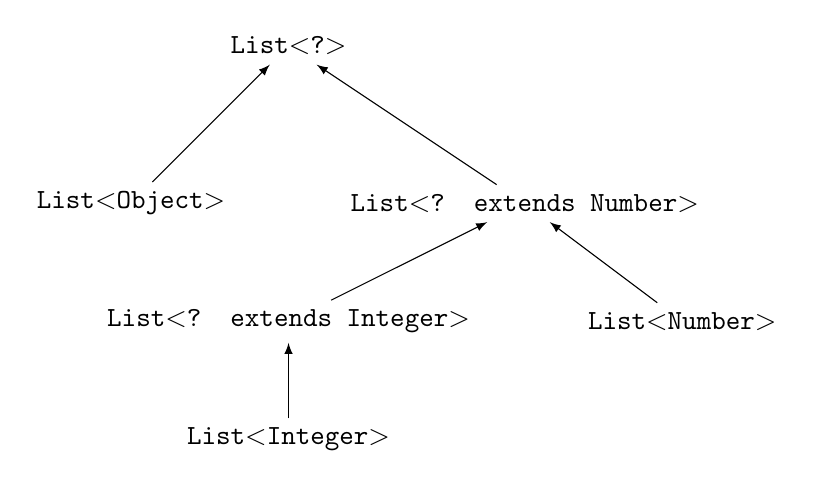
\begin{tikzpicture}{every node/.style={anchor=center}}
    \node (l) at (0,5) {\tt List$<$?$>$} ;
    \node (lo) at (-2,3) {\tt List$<$Object$>$};
    \node (len) at (3,3) {\tt List$<$? extends Number$>$};
    \node (ln) at (5,1.5) {\tt List$<$Number$>$};
    \node (lei) at (0,1.5) {\tt List$<$? extends Integer$>$};
    \node (li) at (0,0) {\tt List$<$Integer$>$};
    \draw[->,>=latex] (li) -- (lei);
    \draw[->,>=latex] (lei) -- (len);
    \draw[->,>=latex] (ln) -- (len);
    \draw[->,>=latex] (len) -- (l);
    \draw[->,>=latex] (lo) -- (l);
  \end{tikzpicture}
\end{figure}

\end{frame}

\begin{frame}{Referência}{}
  \begin{thebibliography}{}
%    \javalangref
  \end{thebibliography}
\end{frame}


